\documentclass{ieeeaccess}
\usepackage{cite}
\usepackage{amsmath,amssymb,amsfonts}
\usepackage{algorithmic}
\usepackage{graphicx}
\usepackage{textcomp}
\usepackage{booktabs}

\newcommand{\RstarNoSetup}{13.71}
\newcommand{\RstarSetup}{15.0}
\newcommand{\QGreedyDet}{297}
\newcommand{\QCtrlDet}{21}
\newcommand{\QRedirDet}{276}
\newcommand{\QStochGreedyMean}{3025}
\newcommand{\QStochGreedyMax}{6026}
\newcommand{\QStochThrMean}{17.6}
\newcommand{\QStochThrMax}{32}
\newcommand{\QStochThrBenefit}{4.20}
\newcommand{\QDppVFiveMean}{2.3}
\newcommand{\QDppVFiveMax}{15}
\newcommand{\QDppVFiveBenefit}{4.20}
\newcommand{\QDppVTenMean}{4.3}
\newcommand{\QDppVTenMax}{16}
\newcommand{\QDppVTenBenefit}{4.71}
\newcommand{\QDppVTwentyMean}{8.7}
\newcommand{\QDppVTwentyMax}{19}
\newcommand{\QDppVTwentyBenefit}{4.92}
\newcommand{\QDppVFiftyMean}{21.9}
\newcommand{\QDppVFiftyMax}{35}
\newcommand{\QDppVFiftyBenefit}{5.00}
\newcommand{\QDppVHundredMean}{43.8}
\newcommand{\QDppVHundredMax}{61}
\newcommand{\QDppVHundredBenefit}{5.03}
\newcommand{\OdgLeakGate}{74}
\newcommand{\OdgBlockedGate}{11}
\newcommand{\OdgTaintBlocked}{44}
\newcommand{\NqCrossFifty}{12}
\newcommand{\NqCrossTen}{13}
\newcommand{\NSeeds}{10}
\newcommand{\NEpisodes}{1500}
\newcommand{\DqnParams}{4{,}674}
\newcommand{\RewLocal}{-2.07}
\newcommand{\LatLocal}{0.87}
\newcommand{\ViolHighLocal}{0.0}
\newcommand{\RewOffload}{-4.43}
\newcommand{\LatOffload}{1.78}
\newcommand{\ViolHighOffload}{100.0}
\newcommand{\RewRandom}{-3.43}
\newcommand{\LatRandom}{1.28}
\newcommand{\ViolHighRandom}{50.3}
\newcommand{\RewThrOnly}{-2.36}
\newcommand{\LatThrOnly}{1.03}
\newcommand{\ViolHighThrOnly}{45.8}
\newcommand{\RewThrOdg}{-1.99}
\newcommand{\LatThrOdg}{0.90}
\newcommand{\ViolHighThrOdg}{0.0}
\newcommand{\RewRules}{-1.97}
\newcommand{\LatRules}{0.88}
\newcommand{\ViolHighRules}{0.0}
\newcommand{\RewQtab}{-2.42}
\newcommand{\LatQtab}{0.97}
\newcommand{\ViolHighQtab}{27.6}
\newcommand{\RewQtabG}{-1.99}
\newcommand{\LatQtabG}{0.85}
\newcommand{\ViolHighQtabG}{0.0}
\newcommand{\RewDqn}{-1.90}
\newcommand{\LatDqn}{0.84}
\newcommand{\ViolHighDqn}{0.0}
\newcommand{\RewDqnG}{-1.91}
\newcommand{\LatDqnG}{0.84}
\newcommand{\ViolHighDqnG}{0.0}
\newcommand{\RewOracle}{-1.89}
\newcommand{\LatOracle}{0.85}
\newcommand{\ViolHighOracle}{0.0}
\newcommand{\ProbeQHigh}{33.4}
\newcommand{\ProbeQHighMax}{37.2}
\newcommand{\ProbeQFav}{34.4}
\newcommand{\ProbeDqnHigh}{0.0}
\newcommand{\ProbeDqnHighMax}{0.0}
\newcommand{\ProbeDqnFav}{0.0}
\newcommand{\GamZeroQ}{-1.93}
\newcommand{\GamZeroDqn}{-1.91}
\newcommand{\GamHalfQ}{-2.00}
\newcommand{\GamHalfDqn}{-1.91}
\newcommand{\GamNinetyQ}{-2.40}
\newcommand{\GamNinetyDqn}{-1.91}


\usepackage{bm}
\makeatletter
\AtBeginDocument{\DeclareMathVersion{bold}
\SetSymbolFont{operators}{bold}{T1}{times}{b}{n}
\SetSymbolFont{NewLetters}{bold}{T1}{times}{b}{it}
\SetMathAlphabet{\mathrm}{bold}{T1}{times}{b}{n}
\SetMathAlphabet{\mathit}{bold}{T1}{times}{b}{it}
\SetMathAlphabet{\mathbf}{bold}{T1}{times}{b}{n}
\SetMathAlphabet{\mathtt}{bold}{OT1}{pcr}{b}{n}
\SetSymbolFont{symbols}{bold}{OMS}{cmsy}{b}{n}
\renewcommand\boldmath{\@nomath\boldmath\mathversion{bold}}}
\makeatother

\begin{document}
\history{Preprint draft, October 2026. Not peer reviewed.}
\doi{}

\title{Security-Aware Adaptive Computation Offloading in Mobile Edge Computing Using Reinforcement Learning and Deep Q-Networks}
\author{\uppercase{Brindeshwar Sharma}\authorrefmark{1}}
\address[1]{Department of Information Technology, Manipal University Jaipur, Jaipur, India (e-mail: brinde.sharma@gmail.com)}

\markboth
{Sharma: Security-Aware Adaptive Computation Offloading in MEC}
{Sharma: Security-Aware Adaptive Computation Offloading in MEC}

\corresp{Corresponding author: Brindeshwar Sharma (e-mail: brinde.sharma@gmail.com).}

\begin{abstract}
Mobile Edge Computing (MEC) enables resource-constrained mobile devices to offload computation-intensive tasks to nearby edge servers. Existing computation offloading approaches primarily optimise latency, energy consumption, or resource allocation, but often do not consider security constraints and multi-user queue stability within a unified decision framework. This paper studies, in simulation, a security-aware adaptive offloading framework that combines an analytical bandwidth threshold, workload classification, reinforcement learning, Lyapunov drift-plus-penalty queue control, Object Dependency Graph (ODG)-based vulnerability scoring, and a Deep Q-Network (DQN) over a continuous state. The framework derives a break-even bandwidth of \RstarNoSetup~Mbps for time-beneficial offloading. A drift-plus-penalty admission controller bounds the edge queue; in a deterministic illustration it holds the queue at \QCtrlDet{} tasks against \QGreedyDet{} for greedy admission. ODG gating keeps labelled sensitive objects on the device, although a ratio-based score is shown to let transitively dependent objects leak. Over \NSeeds{} random seeds, a DQN behind hard gates reaches a reward of \RewDqnG{} per step, against \RewLocal{} for local execution and \RewRules{} for a rule-based pipeline, while a Q-table at the same discount factor falls to \RewQtab. The study is simulation-only, uses N-Queens as a workload proxy, assumes a single edge server and a reward derived from its own cost model, and these limitations are discussed explicitly.
\end{abstract}

\begin{keywords}
Computation offloading, deep Q-network, Lyapunov optimization, mobile edge computing, object dependency graph, reinforcement learning, security-aware offloading.
\end{keywords}

\titlepgskip=-15pt

\maketitle

\section{Introduction}
\label{sec:introduction}
\PARstart{M}{obile} applications are becoming increasingly computation-intensive due to the rapid growth of artificial intelligence, augmented reality, healthcare monitoring, autonomous systems, and Internet of Things (IoT) services \cite{akherfi2018,mao2017}. Although modern smartphones and edge devices continue to improve in processing capability, they remain constrained by battery capacity, computation resources, thermal limitations, and storage availability. Executing complex workloads entirely on mobile devices can therefore lead to excessive energy consumption, increased latency, and degraded user experience \cite{cuervo2010,chun2011}.

Mobile Edge Computing (MEC) has emerged as an effective paradigm for addressing these limitations by enabling mobile devices to offload computationally intensive tasks to nearby edge servers \cite{lin2019,mao2017}. Unlike traditional cloud computing, MEC places computational resources closer to end users, thereby reducing communication latency and improving responsiveness. Numerous computation offloading strategies have been proposed to determine whether a task should be executed locally on the mobile device or remotely on an edge server. The existing approaches are mainly aimed at reducing latency, energy consumption, maximizing throughput, or optimizing the utilization of resources \cite{akherfi2018,zhang2018,wang2018}.

Although great progress has been made in MEC research, there are still some problems that have not yet been solved. First, many of the offloading frameworks make a number of assumptions about network conditions that are stable and do not adapt dynamically to varying bandwidth availability \cite{cuervo2010,chun2011}. Second, conventional approaches often ignore queue congestion at edge servers, which can significantly increase processing delays under heavy workloads \cite{barbarossa2013,chen2016}. Third, existing offloading approaches focus on performance metrics and ignore security and privacy issues of sensitive data offloading to external infrastructures \cite{zhu2013,gan2023}. Finally, traditional Q-Learning-based offloading methods rely on discrete lookup tables that struggle to scale when the state space becomes continuous and high-dimensional \cite{kiran2020,tang2022,huang2019}.

To address these limitations, this paper studies a security-aware adaptive computation offloading framework that integrates analytical modelling, reinforcement learning, queue stability control, vulnerability-aware decision making, and deep reinforcement learning. The framework first derives an analytical break-even bandwidth threshold that determines when offloading becomes beneficial. Computational workloads are characterised with the N-Queens benchmark problem to distinguish lightweight and heavyweight tasks. A Q-Learning agent learns adaptive offloading policies from battery level and workload characteristics, while a Lyapunov drift-plus-penalty controller maintains queue stability in multi-user edge environments.

The framework also includes a security-aware decision layer that is implemented using Object Dependency Graph (ODG) analysis. Application objects receive vulnerability scores based on the access they have to sensitive data such as user identity, medical records, location data, and biometric data. Highly sensitive items are not offloaded, and hence privacy risks and information leakage are lowered. The framework further extends conventional Q-Learning by incorporating a Deep Q-Network (DQN) that can be applied to continuous state spaces, such as battery level, task complexity, vulnerability score, available bandwidth and server load.

This work can be summarized as follows:
\begin{itemize}
\item An analytical bandwidth threshold model for determining the conditions under which edge offloading is beneficial.
\item A workload-aware computation offloading framework that uses reinforcement learning for adaptive decision making.
\item A Lyapunov drift-plus-penalty admission controller for the edge queue in multi-user MEC environments, with a simple queue-length bound.
\item ODG-based vulnerability scoring for security-aware offloading decisions, together with a measurement of how often such a gate leaks on random dependency graphs.
\item An extension of tabular Q-Learning to a Deep Q-Network that handles a continuous state, compared against tabular Q-Learning and rule-based baselines over multiple random seeds.
\end{itemize}
All results come from a simulator; the code, raw outputs and the scripts that generate every figure and table in this paper are available in the accompanying repository.\footnote{\textit{github.com/brindeshwar/security-aware-mec-offloading}}

The remainder of this paper is organized as follows. Section~\ref{sec:related} reviews existing literature on MEC offloading and reinforcement learning approaches. Section~\ref{sec:model} presents the system model and optimization objective. Section~\ref{sec:algorithm} describes the proposed adaptive offloading algorithm. Section~\ref{sec:setup} discusses the experimental configuration. Sections~\ref{sec:workload} through~\ref{sec:dqn} describe workload classification, queue stability, security-aware offloading, and the DQN extension. Section~\ref{sec:results} presents the results and discussion, followed by complexity analysis, limitations, conclusion, and future scope.

\section{Related Work}
\label{sec:related}
Computation offloading has received extensive research in both the Mobile Cloud Computing and the Mobile Edge Computing settings. Early work such as CloneCloud, MAUI and MACS showed that mobile applications could be partitioned and their execution moved to remote servers to save energy and reduce execution time \cite{kovachev2012,cuervo2010,chun2011}. While these early frameworks laid the groundwork for the offloading paradigm, they did not have adaptive intelligence, multi-user queue control or any type of security-aware decision making.

\subsection{Analytical Offloading and Threshold-Based Offloading}
Lin \emph{et al.} survey computation offloading toward edge computing, including wireless-channel and execution-time based criteria for binary offloading decisions \cite{lin2019}. Kovachev and Klamma applied the N-Queens benchmark to the MACS framework to measure the offloading benefit for different task sizes, showing that costly computations benefit significantly from remote execution, while small tasks are dominated by network overhead \cite{kovachev2012}. These analytical methods offer clear decision criteria, but are not able to account for the changing state of the battery, changing workload, or sensitivity of the data being offloaded.

\subsection{Reinforcement Learning for Adaptive Offloading}
Kiran \emph{et al.} introduced a Software Defined Edge Cloudlet framework with the aid of Q-Learning for joint resource allocation and computation offloading, showing that reinforcement learning can outperform greedy and random strategies in minimizing delay \cite{kiran2020}. Huang \emph{et al.} further built on this research with a deep reinforcement learning algorithm for joint task offloading and bandwidth allocation in multi-user MEC systems that demonstrated higher performance under different channel conditions \cite{huang2019}. Tang and Wong presented a model-free distributed algorithm based on deep reinforcement learning that allows each device to make offloading decisions without knowing the state of other devices, or the task models \cite{tang2022}. Later, He \emph{et al.} investigated multi-agent deep reinforcement learning for dynamic task offloading in D2D-MEC networks to reduce the average task delay while meeting the deadline requirements of distributed decision makers \cite{he2024}.

\subsection{Queue Stability and Congestion Control}
Bi \emph{et al.} proposed a deep reinforcement learning framework with Lyapunov guidance (LyDROO) to solve the online computation offloading problem in MEC networks with long-term queue and power constraints, which significantly outperforms the greedy baseline in multi-user MEC networks \cite{bi2021}. Bae \emph{et al.} also theoretically linked reinforcement learning to Lyapunov optimization, establishing a link between stability guarantees and learned policies \cite{bae2020}. In this direction, Chen \emph{et al.} directly addressed multi-user contention for edge resources and proposed efficient decentralized offloading game formulations for mobile-edge cloud computing \cite{chen2016}. Wang \emph{et al.} optimized the energy consumption and latency of offloading and computing in wireless powered MEC systems with energy constraints while considering multi-user resource sharing, where they showed energy-latency tradeoffs \cite{wang2018}.

\subsection{Security and Privacy in Offloading Decisions}
Although performance improvements have been made, few offloading frameworks have taken security into account. Zhu \emph{et al.} presented Object Dependency Graphs for vulnerability assessment of mobile applications offloaded to cloud infrastructure, which identifies the sensitive objects and their inter-dependencies \cite{zhu2013}. Their method models application-level privacy risk in the offloading context, but was static and not used with any reinforcement learning or queue stability mechanism. Gan \emph{et al.} took privacy concerns a step further by introducing differentially private deep Q-learning for pattern privacy preservation in MEC offloading, where they demonstrated that privacy guarantees can be incorporated into the learning objective \cite{gan2023}. Zhao \emph{et al.} used deep Q-networks to solve the task offloading problem in a cooperative intrusion detection system and showed that the security-functional workload can be scheduled at the edge \cite{zhao2022}.

\subsection{Continuous-State Learning and Deep Q-Networks}
Zhang \emph{et al.} proposed an optimization of the energy-latency trade-off in MEC under different network conditions based on analytical energy models \cite{zhang2018}. Mao \emph{et al.} gave a comprehensive study from the communication perspective, setting the system models and optimization goals for many of the following DRL-based offloading studies \cite{mao2017}. Yang \emph{et al.} used DQN-based task offloading for multimedia data analysis in edge-computing-enabled Internet of Vehicles (IoV) to support decision making in multi-variety task environments \cite{yang2022}. Anand and Karthikeyan proposed an Adaptive and Intelligent Customized DQN (AICDQN) for priority-aware, energy-efficient task scheduling in MEC, demonstrating that customized DQN formulations can yield better performance than standard ones on dynamic IoT workloads \cite{anand2026}.

\subsection{Dependency-Aware and Graph-Based Offloading}
Recent efforts have turned to explicitly modelling task interdependencies. Liu \emph{et al.} introduced an online task offloading strategy for IoV with DRL that optimizes task latency and energy consumption based on cooperative base stations and edge servers and considers the task dependency graph \cite{liu2024dep}. A similar approach was proposed for dependency-aware dynamic offloading in multi-device MEC, where the execution of local tasks is adjusted according to the status of edge nodes and the precedence of the tasks under time-varying fading channels (the DODA-DT algorithm) \cite{fang2024}. The DCEDRL method extended this work by introducing density clustering and ensemble learning with DRL for the offloading decision, which uses multiple neural networks trained together to alleviate the sensitivity to dynamic channel and load changes \cite{qin2025}. A parallel approach with asynchronous training and parallel exploration was shown to improve convergence stability for multi-user offloading decisions in dynamic edge environments \cite{chen2025mon}.

\subsection{Recent Advances: Temporal, Cooperative and Intelligent Frameworks}
Zhang \emph{et al.} discussed that time-ordered task graphs need special scheduling policies other than the standard Markov-state formulations \cite{zhang2025}. For large-scale dynamic workloads, Sun \emph{et al.} proposed a three-layer cloud-edge-device task offloading model based on DRL, which has advantages over two-layer architectures \cite{sun2026}. Jalal \emph{et al.} proposed Public Edge as a Service (PEaaS) as an intermediate layer and designed a PPO-based scheduler, which includes mobility, congestion, cost and energy in a single reward function for intelligent regional offloading \cite{jalal2026}. Dependent-task offloading with DRL has also been studied for general edge computing \cite{wang2022dep}. Table~\ref{tab:compare} summarizes the capabilities of existing MEC offloading frameworks against the framework studied here across seven dimensions.

\subsection{Summary of Gaps}
It has been found from the literature that current computation offloading frameworks consider only a subset of the decision factors necessary for real-world MEC deployment. Previous works have individually investigated bandwidth-aware offloading, reinforcement learning, Lyapunov-based queue control, security-aware computation, and deep reinforcement learning; however, few studies have combined these techniques into a unified end-to-end decision-making framework. Motivated by this gap, we study an adaptive offloading framework that integrates bandwidth thresholding, workload-aware learning, queue stability control, ODG-based vulnerability analysis, and DQN-based continuous-state optimization, and we evaluate it against explicit baselines.

\begin{table*}[t]
\caption{Qualitative comparison of MEC offloading frameworks. Each cell reflects the focus stated in the cited work, as read by the author, and is not a quantitative benchmark. ``Yes'' means the dimension is addressed, ``Partial'' that it is addressed only in part, and ``Static'' that security is assessed offline only. The last row describes the framework studied in this paper, in simulation.}
\label{tab:compare}
\centering
\footnotesize
\begin{tabular}{@{}p{5.3cm}cccccccc@{}}
\toprule
Framework & Latency & Energy & AI-driven & Queue & Security- & Continuous & Dependency- \\
 & opt. & opt. & & stability & aware & state & aware \\
\midrule
CloneCloud, MAUI, MACS \cite{kovachev2012,cuervo2010,chun2011} & Yes & Yes & No & No & No & No & No \\
Lin \emph{et al.} \cite{lin2019} & Yes & No & No & No & No & No & No \\
Barbarossa \emph{et al.}, Bi \emph{et al.} \cite{barbarossa2013,bi2021} & Yes & Yes & Partial & Yes & No & No & No \\
Kiran \emph{et al.}, Huang \emph{et al.} \cite{kiran2020,huang2019} & Yes & Yes & Yes & No & No & No & No \\
Tang \& Wong, He \emph{et al.} \cite{tang2022,he2024} & Yes & Yes & Yes & No & No & Yes & No \\
Zhu \emph{et al.}, Zhao \emph{et al.} \cite{zhu2013,zhao2022} & No & No & Partial & No & Static & No & No \\
Gan \emph{et al.} \cite{gan2023} & Yes & Yes & Yes & No & Yes & No & No \\
Yang \emph{et al.}, Anand \& Karthikeyan \cite{yang2022,anand2026} & Yes & Yes & Yes & No & No & Yes & No \\
Liu \emph{et al.}, Fang \emph{et al.}, Wang \emph{et al.} \cite{liu2024dep,fang2024,wang2022dep} & Yes & Yes & Yes & No & No & Yes & Yes \\
\textbf{This work (simulation)} & Yes & Yes & Yes & Yes & Yes & Yes & Yes \\
\bottomrule
\end{tabular}
\end{table*}

\section{System Model}
\label{sec:model}
The proposed system consists of a mobile device, an edge server, a wireless communication link, and a decision engine. Each incoming task is evaluated using network conditions, task complexity, battery level, vulnerability score, and server load.

\subsection{Local Execution Model}
For a task requiring $n$ CPU cycles and a local device frequency $f_\text{local}$, the local execution time is
\begin{equation}
T_\text{local} = \frac{n}{f_\text{local}}.
\end{equation}

\subsection{Edge Offloading Model}
For a task with input data size $m$ bits, transmission rate $R$, and edge-server frequency $f_\text{remote}$, the offloading time is
\begin{equation}
T_\text{offload} = \frac{m}{R} + \frac{n}{f_\text{remote}} \;(+\, T_\text{setup} + T_\text{queue}).
\end{equation}
The terms in parentheses are the connection setup delay and the waiting time at a loaded edge server; they are zero in the analytical derivation and non-zero in the simulation (Section~\ref{sec:setup}). Offloading is beneficial when $T_\text{offload} < T_\text{local}$. Solving for the break-even bandwidth gives
\begin{equation}
R^{*} = \frac{m}{\dfrac{n}{f_\text{local}} - \dfrac{n}{f_\text{remote}}}.
\label{eq:threshold}
\end{equation}
Using $n = 10^{9}$ cycles, $m = 8$~Mb, $f_\text{local} = 1.2$~GHz, and $f_\text{remote} = 4.0$~GHz, the break-even bandwidth is $R^{*} = \RstarNoSetup$~Mbps. Including the 50~ms setup delay moves the break-even point to $\RstarSetup$~Mbps. This threshold acts as the first decision gate: if the available bandwidth is below $R^{*}$, the task is executed locally. Fig.~\ref{fig:breakeven}(a) shows the two completion-time curves and their crossing points for the reference task. Fig.~\ref{fig:breakeven}(b) shows how $R^{*}$ moves with the edge speed-up and the setup delay: a faster edge lowers the threshold, while a longer setup delay raises it sharply as the speed-up approaches one.

\begin{figure*}[t]
\centering
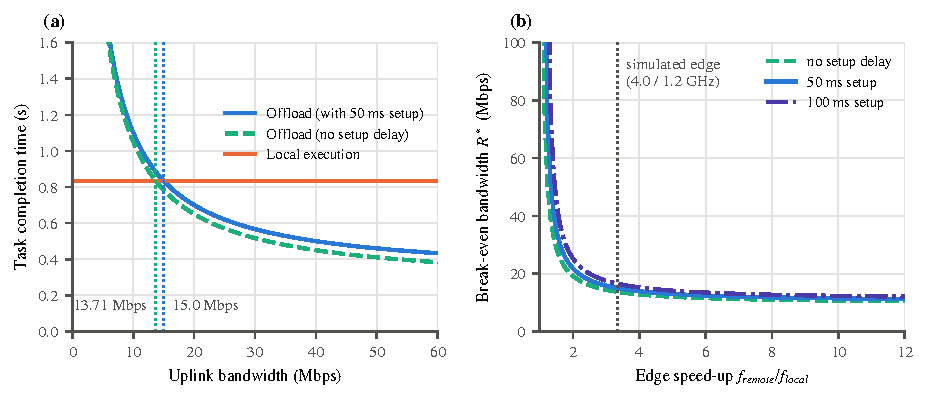
\includegraphics[width=\textwidth]{../results/figures/fig01_breakeven.pdf}
\caption{Analytical break-even bandwidth. (a)~Completion time of the reference task (1 Gcycle, 8~Mb) versus uplink bandwidth: local execution (orange, constant), offloading without setup delay (green, dashed) and with a 50~ms setup delay (blue). The curves cross at $\RstarNoSetup$ and $\RstarSetup$~Mbps (dotted lines). (b)~Break-even bandwidth $R^{*}$ as a function of the edge-to-device frequency ratio for three setup delays; the dotted line marks the simulated ratio $4.0/1.2$.}
\label{fig:breakeven}
\end{figure*}

\subsection{Energy Model}
Local energy consumption is modelled as
\begin{equation}
E_\text{local} = P_\text{cpu}\, T_\text{local},
\end{equation}
and the device-side energy of offloading as
\begin{equation}
E_\text{offload} = P_\text{tx}\, T_\text{tx} + P_\text{idle}\, T_\text{wait},
\end{equation}
where $P_\text{tx}$ is the transmission power, $T_\text{tx}=m/R$, and $P_\text{idle}$ is the idle power while waiting for the remote execution ($T_\text{wait}$ covers setup, edge computation and queueing). The simulation uses $P_\text{cpu}=0.9$~W, $P_\text{tx}=1.3$~W and $P_\text{idle}=0.15$~W; these are assumed values, not measurements.

\subsection{Optimization Objective}
The framework jointly considers latency, energy consumption, queue congestion, and security. Latency, energy and security enter the per-task reward that the learning agents maximise,
\begin{equation}
r = -\bigl(T + \beta(b)\,E\bigr) - a\,\sigma(V),
\label{eq:reward}
\end{equation}
where $a\in\{0,1\}$ is the decision (1 = offload), $b\in[0,1]$ is the battery level, $\beta(b) = 0.5\,(1+3(1-b))$ weights energy more heavily as the battery drains, and $\sigma(V)$ is a penalty for offloading a task with vulnerability score $V$: $\sigma=0$ for $V<0.33$, $1.5$ for $0.33\le V<0.66$ and $3.0$ for $V\ge0.66$. Queue congestion enters through the edge load, which raises $T_\text{queue}$ for later tasks, and through the explicit admission controller of Section~\ref{sec:queue}. When the battery reaches zero the episode ends with an extra penalty of 5.

\section{Proposed Algorithm}
\label{sec:algorithm}
The proposed algorithm performs a sequence of decision checks before a task is either executed locally or offloaded to the edge server. The decision process is designed to ensure that offloading occurs only when it is beneficial, secure, and stable from the perspective of the edge infrastructure.
\begin{enumerate}
\item Receive the incoming task request.
\item Measure the available bandwidth.
\item Compare the bandwidth with the break-even threshold; if it is lower, execute locally.
\item Compute the ODG vulnerability score of the task's objects.
\item If the score is at or above the gate $\tau_V$, force local execution.
\item Otherwise evaluate the learned policy (Q-Learning or DQN), whose input includes the task complexity, the battery level and the edge load.
\item Check the edge load; if it is at or above the load limit $\Lambda$, execute locally.
\item Otherwise offload the task to the edge server.
\end{enumerate}
Fig.~\ref{fig:pipeline} shows the gates in order. The workload classification of Section~\ref{sec:workload} characterises how task size affects the offloading benefit; in the implemented pipeline it is carried by the complexity input of the learned policy. The multi-user admission controller of Section~\ref{sec:queue} regulates how many offloaded tasks reach the edge queue per slot, and is evaluated separately.

\begin{figure*}[t]
\centering
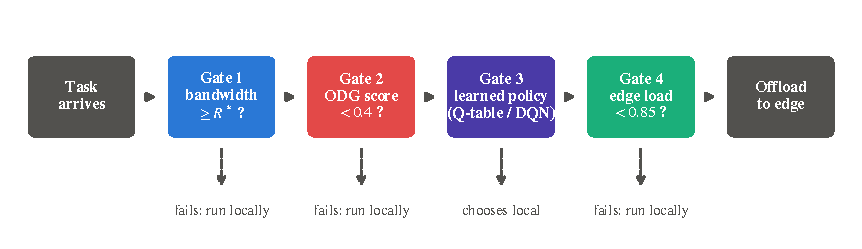
\includegraphics[width=\textwidth]{../results/figures/fig03_pipeline.pdf}
\caption{The decision pipeline as implemented. A task is offloaded only if it passes the bandwidth gate ($R\ge R^{*}$), the ODG gate (score below $\tau_V=0.4$), the learned policy, and the edge-load gate (load below $\Lambda=0.85$); failing any gate, or a ``local'' decision by the learned policy, executes the task on the device.}
\label{fig:pipeline}
\end{figure*}

\begin{center}
\begin{minipage}{0.95\columnwidth}
\footnotesize
\textbf{Algorithm 1:} Offloading decision for one task.
\begin{algorithmic}[1]
\STATE \textbf{Input:} bandwidth $R$, vulnerability $V$, battery $b$, complexity $c$, edge load $\ell$
\IF{$R < R^{*}$ \OR $V \ge \tau_V$ \OR $\ell \ge \Lambda$}
\STATE \textbf{return} local
\ENDIF
\STATE $a \leftarrow \arg\max_{a'} Q(s, a')$ \COMMENT{Q-table or DQN}
\STATE \textbf{return} offload if $a = 1$, otherwise local
\end{algorithmic}
\end{minipage}
\end{center}

\section{Experimental Setup}
\label{sec:setup}
\subsection{Simulation Environment}
The framework was implemented in Python using NumPy and Matplotlib, including the DQN, whose forward and backward passes are written by hand. All experiments run on a single workstation; the full set of experiments takes roughly twenty minutes. The MEC environment consists of a mobile device operating at 1.2~GHz and an edge server operating at 4.0~GHz. A task of complexity $c\in(0,1]$ requires $n = c\cdot 2\times10^{9}$ cycles and $m = c\cdot 16$~Mb of input data, so that $c=0.5$ is the reference task (one billion cycles, 8~Mb); because $n$ and $m$ scale together, the break-even bandwidth of Eq.~\eqref{eq:threshold} does not depend on $c$. A fixed network setup delay of 50~ms represents connection initialization overhead. The bandwidth follows a log-random walk between 1 and 100~Mbps. The edge load $\ell\in[0,1]$ rises with offloaded work and decays otherwise, and adds a queueing delay of $0.8\,\ell^{2}$ seconds, so that offloading has a cost for later tasks. Task complexity $c$ is drawn uniformly from $(0.05,1]$ and the vulnerability score $V$ from a Beta$(1,2)$ distribution (most tasks are low-risk; about 12\% have $V\ge0.66$). An episode ends after 60 tasks or when the battery reaches zero.

\subsection{Learning Configuration}
Table~\ref{tab:params} lists the configuration. The Q-table sees the same observation as the DQN after discretisation (5 battery levels, 4 complexity levels, 3 vulnerability buckets, 6 bandwidth bins and 4 load levels, 1{,}440 states). The DQN is a $5\to64\to64\to2$ ReLU network with \DqnParams{} weights, experience replay, a target network and the Adam optimizer. Both agents are trained for \NEpisodes{} episodes on each of \NSeeds{} random seeds and are evaluated greedily on 200 fresh episodes per seed, generated from a random stream that is shared by all policies of the same seed.

\begin{table}[t]
\caption{Configuration of the simulation and of the learning agents. Power and battery values are assumptions chosen to be plausible, not measurements.}
\label{tab:params}
\centering
\footnotesize
\begin{tabular}{@{}p{4.1cm}p{4.2cm}@{}}
\toprule
Parameter & Value \\
\midrule
Device / edge CPU & 1.2 GHz / 4.0 GHz \\
Setup delay, bandwidth range & 50 ms, 1--100 Mbps \\
Power: CPU / transmit / idle & 0.9 W / 1.3 W / 0.15 W \\
Battery budget & 60 J \\
Security penalty $\sigma$ (MED / HIGH) & 1.5 / 3.0 \\
ODG gate $\tau_V$, load limit $\Lambda$ & 0.4, 0.85 \\
Discount factor $\gamma$ & 0.95 \\
Q-table learning rate & 0.1 \\
DQN learning rate (Adam) & 0.001 \\
DQN replay buffer / batch & 20{,}000 / 64 \\
DQN target-network update & every 200 steps \\
Exploration $\epsilon$ & 1.0 to 0.05, linear over first 60\% of episodes \\
Training episodes, seeds & \NEpisodes{}, \NSeeds{} \\
Queue: arrival / capacity & Poisson(10) / 7 tasks per slot \\
\bottomrule
\end{tabular}
\end{table}

\subsection{Baselines and Metrics}
Every learned policy is compared with simple policies: \emph{always local}, \emph{always offload} (greedy), \emph{random}, \emph{threshold only} (offload iff $R\ge R^{*}$), \emph{threshold plus ODG gate}, and a \emph{rule pipeline} that adds the load gate. A \emph{myopic oracle}, which picks the action with the higher immediate reward using the true model, serves as a reference that is not realisable without knowing the model. We report the reward per step, the latency and energy per task, the share of offloaded tasks, the share of high-vulnerability tasks ($V\ge0.66$) that were offloaded, and the share of episodes that deplete the battery, each as a mean over seeds with a 95\% confidence interval.
\section{Workload Classification and Q-Learning}
\label{sec:workload}
The first intelligent decision layer of the framework is based on workload characterisation and reinforcement learning. Since lightweight and heavyweight computational tasks exhibit significantly different execution characteristics, a workload-aware policy is required before deciding whether a task should be executed locally or offloaded \cite{kiran2020,huang2019}.

\subsection{N-Queens Workload Proxy}
To emulate computational workloads with varying complexity, the N-Queens problem was adopted as a CPU-bound proxy. It is used in computation offloading research because the computational cost increases rapidly with problem size while maintaining a consistent problem structure \cite{kovachev2012}. Here the task is to count all solutions of the $N$-Queens problem with a bitmask backtracking solver; the local time is measured on the machine running the simulation (median of three runs), and the edge time is \emph{modelled}, not measured: the local time scaled by the CPU ratio $f_\text{local}/f_\text{remote}$, plus the 50~ms setup delay and the time to send 8~Mb at the given bandwidth. Tasks with small $N$ are classified as lightweight, since the setup and transfer overhead exceeds the compute saving, whereas larger $N$ are heavyweight. Fig.~\ref{fig:nqueens} shows that the modelled edge execution overtakes local execution at $N=\NqCrossFifty$ on a 50~Mbps link and at $N=\NqCrossTen$ on a 10~Mbps link, so a slower link moves the crossover to heavier tasks. Because local times are measured on a desktop CPU rather than on a phone, the absolute values and the crossover $N$ depend on the machine; the figure illustrates the shape of the trade-off rather than a device measurement.

\begin{figure}[t]
\centering
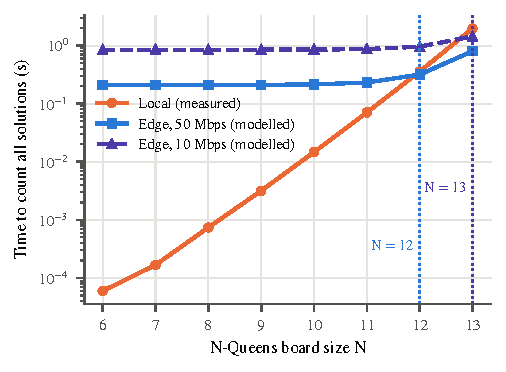
\includegraphics[width=\columnwidth]{../results/figures/fig02_nqueens.pdf}
\caption{N-Queens workload proxy (log scale). Measured local time to count all solutions (orange) versus the modelled edge time at 50~Mbps (blue) and 10~Mbps (violet dashed). Dotted lines mark the first board size at which the edge becomes faster. Edge times are modelled from the local time, the CPU ratio, a 50~ms setup delay and the transfer of 8~Mb; they are not measured on a remote machine.}
\label{fig:nqueens}
\end{figure}

\subsection{Tabular Q-Learning Agent}
The tabular agent observes five quantities, discretised: battery level, task complexity, vulnerability bucket, bandwidth relative to the threshold, and edge load. The available actions are to execute locally or to offload to the edge server. The objective of the Q-Learning agent is to maximize the long-term cumulative reward \cite{kiran2020}:
\begin{equation}
Q(s,a) \leftarrow Q(s,a) + \alpha\bigl[r + \gamma \max_{a'} Q(s',a') - Q(s,a)\bigr],
\label{eq:qupdate}
\end{equation}
where $Q(s,a)$ is the state-action value, $\alpha$ is the learning rate, $\gamma$ is the discount factor, $r$ is the immediate reward of Eq.~\eqref{eq:reward} and $s'$ is the next state. The reward trades latency and energy against the security penalty. The environment is dynamic: the battery drains with every task, the edge load increases when tasks are offloaded, and the bandwidth moves, so that an offloading decision affects the later states. The agent learns by interacting with this environment and gradually modifying its policy \cite{tang2022,huang2019}. How quickly it learns, and how well, is examined in Section~\ref{sec:results} using the reward of the greedy policy on fresh episodes; unlike the sum of Q-values, this quantity directly shows whether the policy is improving.

\section{Queue Stability Using Lyapunov Control}
\label{sec:queue}
While reinforcement learning can detect beneficial offloading opportunities, aggressive offloading can cause edge servers to be overloaded, with resulting queue growth. To overcome this challenge, a Lyapunov drift-plus-penalty admission controller is added to the framework \cite{bi2021,bae2020}.

\subsection{Controller}
Let $Q(t)$ be the length of the edge queue at time slot $t$, $a(t)$ the number of tasks admitted to the edge and $\mu$ the number of tasks served per slot, so that $Q(t+1)=\max\{Q(t)+a(t)-\mu,\,0\}$. The Lyapunov function and drift are
\begin{equation}
L(Q(t)) = \tfrac12 Q(t)^2,
\end{equation}
\begin{equation}
\Delta(Q(t)) = \mathbb{E}\bigl[L(Q(t+1)) - L(Q(t))\mid Q(t)\bigr].
\end{equation}
To maintain queue stability the controller minimizes the drift-plus-penalty expression
\begin{equation}
\Delta(Q(t)) + V\cdot\text{Penalty}(t),
\label{eq:dpp}
\end{equation}
where $V$ is a control parameter that balances queue stability against performance. Each arriving task $i$ has an offloading benefit $b_i\in(0,b_\text{max}]$ (for example, the latency it saves relative to local execution), so the penalty is $-\sum_{i\text{ admitted}} b_i$. Since $\Delta(Q) \le B + Q(t)\,\mathbb{E}[a(t)-\mu\mid Q(t)]$ for a constant $B$, minimizing the bound in each slot gives a simple rule: admit task $i$ if and only if
\begin{equation}
V\, b_i > Q(t),
\label{eq:admit}
\end{equation}
and execute it locally otherwise.

\textbf{Queue bound.} With $b_i\le b_\text{max}$ and at most $A_\text{max}$ admitted tasks per slot, $Q(t)\le V b_\text{max} + A_\text{max}$ for all $t$. Proof: if $Q(t)\ge V b_\text{max}$, rule~\eqref{eq:admit} admits no task, so $Q$ cannot increase in that slot; $Q$ can therefore exceed $V b_\text{max}$ only by the tasks admitted in a single slot, at most $A_\text{max}$. The parameter $V$ trades queue length against the benefit gained: a larger $V$ admits more tasks at the cost of a longer queue.

\subsection{Results}
We evaluate the controller in two settings (Fig.~\ref{fig:queue} and Table~\ref{tab:queue}). The first is the deterministic illustration used earlier in this study: 10 tasks arrive per slot, the server serves 7, and a simple throttle admits only 4 tasks per slot once the queue reaches 20. Over 100 slots, greedy admission grows by $10-7=3$ tasks per slot and ends at $\QGreedyDet$ tasks ($3\times99$), whereas the throttled queue stays at a maximum of $\QCtrlDet$ and redirects $\QRedirDet$ tasks to local execution (Fig.~\ref{fig:queue}a). The value $\QGreedyDet$ is a consequence of the chosen rates and horizon; it illustrates that greedy admission is unbounded when arrivals exceed capacity, and the boundedness of the throttled queue follows directly from its rule.

The second setting is stochastic: Poisson arrivals with mean 10 per slot, benefits $b_i\sim U(0.2,1)$, service capacity 7 per slot, 2{,}000 slots and 20 seeds. Greedy admission reaches a mean queue of $\QStochGreedyMean$ tasks, while the fixed threshold of 20 keeps a mean of $\QStochThrMean$ and a maximum of $\QStochThrMax$ because Poisson bursts overshoot it. The drift-plus-penalty rule with $V=20$ holds the mean at $\QDppVTwentyMean$ and the maximum at $\QDppVTwentyMax$, within the bound $V b_\text{max}+A_\text{max}$, while collecting a benefit of $\QDppVTwentyBenefit$ per slot compared with $\QStochThrBenefit$ for the fixed threshold. Both controllers admit about 70\% of arrivals (the service capacity), but drift-plus-penalty chooses the higher-benefit tasks. Increasing $V$ raises both the mean queue and the benefit, with diminishing returns (Fig.~\ref{fig:queue}c).

\begin{figure*}[t]
\centering
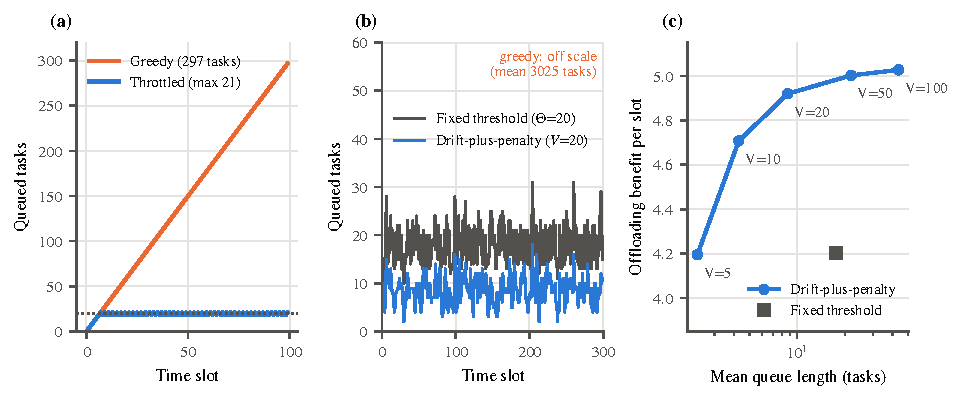
\includegraphics[width=\textwidth]{../results/figures/fig05_queue.pdf}
\caption{Edge-queue control. (a)~Deterministic illustration: constant arrivals (10 per slot) exceed the capacity (7 per slot); greedy admission grows linearly to 297 tasks after 100 slots while the throttle keeps the queue at most 21 (dotted line: threshold 20). (b)~Stochastic arrivals (Poisson, mean 10), first 300 slots of one seed: the fixed threshold overshoots in bursts, drift-plus-penalty with $V=20$ keeps the queue shorter; greedy admission is off scale. (c)~Trade-off between mean queue length (log axis) and offloading benefit per slot as $V$ varies (mean over 20 seeds), with the fixed threshold for reference.}
\label{fig:queue}
\end{figure*}

\begin{table}[t]
\caption{Edge-queue control under stochastic arrivals (Poisson, mean 10 per slot; capacity 7 per slot; 2{,}000 slots; mean over 20 seeds). DPP is drift-plus-penalty. ``Admitted'' is the share of arriving tasks sent to the edge; ``benefit'' is the summed offloading benefit of admitted tasks per slot (mean $\pm$ 95\% CI).}
\label{tab:queue}
\centering
\footnotesize
\setlength{\tabcolsep}{3.5pt}
\begin{tabular}{@{}lrrrr@{}}
\toprule
Policy & Mean $Q$ & Max $Q$ & Admitted (\%) & Benefit/slot \\
\midrule
Greedy & 3024.5 & 6026 & 100 & 6.00 $\pm$ 0.02 \\
Threshold $\Theta=20$ & 17.6 & 32 & 70 & 4.20 $\pm$ 0.01 \\
DPP, $V=5$ & 2.3 & 15 & 66 & 4.20 $\pm$ 0.01 \\
DPP, $V=10$ & 4.3 & 16 & 70 & 4.71 $\pm$ 0.01 \\
DPP, $V=20$ & 8.7 & 19 & 70 & 4.92 $\pm$ 0.01 \\
DPP, $V=50$ & 21.9 & 35 & 70 & 5.00 $\pm$ 0.01 \\
DPP, $V=100$ & 43.8 & 61 & 70 & 5.03 $\pm$ 0.01 \\
\bottomrule
\end{tabular}

\end{table}

\section{Security-Aware Offloading}
\label{sec:odg}
Most computation offloading frameworks consider only latency and energy efficiency. However, many mobile applications process highly sensitive information such as personal identifiers, healthcare records, location information, and biometric measurements. Offloading such data without considering the security implications can introduce significant privacy risks \cite{akherfi2018,gan2023}.

To address this challenge, the framework introduces an Object Dependency Graph (ODG)-based vulnerability scoring mechanism. The ODG models application objects and their dependencies. Objects that directly access sensitive information are assigned the highest vulnerability score \cite{zhu2013}.

\subsection{Vulnerability Score and Gate}
The vulnerability score of an object $i$ is defined as the share of the objects reachable from it that are sensitive,
\begin{equation}
V_i = \frac{\text{sensitive objects reachable from } i}{\text{all objects reachable from } i},\qquad 0\le V_i\le1,
\label{eq:vuln}
\end{equation}
computed by depth-first search over transitive dependencies; a sensitive object has $V_i=1$. $V_i=0$ indicates that the object does not depend on sensitive data and can be offloaded, and $V_i=1$ indicates a highly sensitive object. The vulnerability score is incorporated into the offloading decision in two ways. First, a hard gate: objects with $V_i\ge\tau_V=0.4$ are never offloaded, regardless of bandwidth availability or the learned policy. Second, the learned agents see $V$ as an input and receive the security penalty $\sigma(V)$ of Eq.~\eqref{eq:reward} with the thresholds Low ($V<0.33$), Medium ($0.33\le V<0.66$) and High ($V\ge0.66$).

\subsection{Example Application}
The example application is a hand-built healthcare/fitness app with twelve objects: four sensitive ones (user ID, heart rate, medical record, location), four safe utilities and four composite objects (Fig.~\ref{fig:odg}a). All four sensitive objects score 1.0 and stay on the device; this follows from their labelling together with a hard rule, so it is a property of the gate rather than an empirical result. The composite objects \emph{analyzeHealth} and \emph{buildReport} score 0.50 and stay local, whereas \emph{syncToCloud} (0.29) and \emph{runAIInference} (0.33) fall below the gate and may be offloaded. Note that \emph{syncToCloud} depends on \emph{getUserID} through \emph{buildReport}; the ratio of Eq.~\eqref{eq:vuln} dilutes this dependency because the object also reaches several safe ones.

\subsection{A Stricter Taint Gate and Its Cost}
To quantify this effect we compare the ratio score with a conservative \emph{taint} score that is 1 whenever an object can reach any sensitive object, and 0 otherwise. On 300 random dependency graphs (30 objects, 20\% sensitive, edge probability 0.12), the paper's gate (ratio score, $\tau_V=0.4$) allows \OdgLeakGate\% of the objects that reach sensitive data to offload while forcing only \OdgBlockedGate\% of the non-sensitive objects to stay local. The taint gate leaks none, at the price of keeping \OdgTaintBlocked\% of the non-sensitive objects local (Fig.~\ref{fig:odg}b). Lowering the ratio threshold moves along the curve between these two points. Which operating point is appropriate depends on the application: the taint gate protects better, but it removes much of the offloadable computation when the dependency graph is dense.

\begin{figure*}[t]
\centering
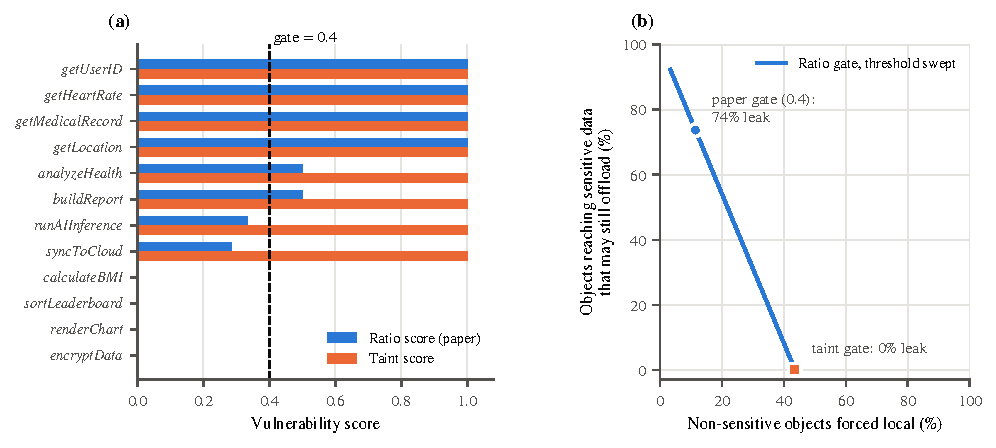
\includegraphics[width=\textwidth]{../results/figures/fig04_odg.pdf}
\caption{ODG vulnerability scoring. (a)~Scores of the twelve objects of the example application under the ratio score of the paper (blue) and the conservative taint score (orange); the dashed line is the gate $\tau_V=0.4$. Objects scoring above it must run locally. \emph{syncToCloud} and \emph{runAIInference} pass the ratio gate although they depend on sensitive objects. (b)~On random dependency graphs, the percentage of objects that reach sensitive data but may still offload (vertical axis) against the percentage of non-sensitive objects forced local (horizontal axis) as the ratio threshold is swept (blue curve). The dot is the gate of the paper ($\tau_V=0.4$); the square is the taint gate.}
\label{fig:odg}
\end{figure*}

\section{Security-Aware Reinforcement Learning}
\label{sec:secrl}
The reward function incorporates the vulnerability score so that the learning agents take security risk into account in addition to latency and energy. The secure reward of Eq.~\eqref{eq:reward} subtracts $\sigma(V)$ whenever a task is offloaded; the higher the risk, the lower the payoff of offloading, which makes the agent more likely to execute sensitive tasks locally and to keep offloading low-risk, computationally heavy tasks when the network allows it. This is a soft constraint: the penalty makes unsafe offloading unattractive but does not forbid it. Whether the learned policies respect it is therefore a measurable question, which we answer in Section~\ref{sec:results} by probing the trained agents on high-vulnerability states, and the hard ODG gate is kept as a separate guarantee in front of the learned policy.

\section{Deep Q-Network Extension}
\label{sec:dqn}
Although Q-Learning performs effectively in small environments, its scalability is limited because state-action values must be stored explicitly in a lookup table, and a continuous state has to be discretised, which merges states that call for different actions. As the number of state variables increases, the Q-table grows exponentially. To overcome this limitation, the framework extends conventional Q-Learning with a Deep Q-Network (DQN): instead of storing explicit state-action values, a neural network is trained to approximate the action-value function \cite{yang2022,anand2026,sun2026}.

The DQN receives five continuous inputs: battery level, task complexity, vulnerability score, available bandwidth (on a log scale) and edge-server load. The network has an input layer of five neurons, two hidden layers of 64 ReLU neurons and an output layer of two actions, and approximates $Q(s,a;\theta)$ with parameters $\theta$ (\DqnParams{} weights in total). It is trained by minimizing the temporal-difference loss \cite{tang2022,yang2022}
\begin{equation}
\mathcal{L}(\theta) = \Bigl(r + \gamma \max_{a'} Q(s',a';\theta^{-}) - Q(s,a;\theta)\Bigr)^{2},
\end{equation}
where $\theta^{-}$ are the parameters of a target network, with a clipped (Huber-style) gradient. Transitions $(s_t,a_t,r_t,s_{t+1})$ are stored in a replay buffer and mini-batches are sampled at random, which breaks the correlation between consecutive experiences; the target network is copied from the online network every 200 steps; and the exploration rate $\epsilon$ decays linearly from 1.0 to 0.05 over the first 60\% of training. Table~\ref{tab:params} gives the configuration.
\section{Results and Discussion}
\label{sec:results}
The framework was evaluated through a series of experiments examining the bandwidth threshold, workload classification, queue control, vulnerability-aware offloading, and the learned decision policies. The bandwidth threshold, queue control and ODG results are reported in Sections~\ref{sec:model}, \ref{sec:queue} and~\ref{sec:odg}; this section compares the decision policies end to end. All numbers are means over \NSeeds{} seeds with 95\% confidence intervals unless stated otherwise.

\subsection{Policy Comparison}
Table~\ref{tab:policies} and Fig.~\ref{fig:policies} compare the policies on 200 fresh episodes per seed. Offloading everything is the worst choice: the edge load saturates and many tasks are sent over slow links, giving a reward of $\RewOffload$ per step against $\RewLocal$ for always executing locally. Offloading whenever the bandwidth exceeds $R^{*}$ improves on greedy offloading but still offloads about 46\% of the tasks, including 46\% of the high-vulnerability ones, and stays below local execution on reward ($\RewThrOnly$). Adding the ODG gate removes the security violations and raises the reward to $\RewThrOdg$, and the load gate raises it slightly further to $\RewRules$ for the complete rule pipeline.

The learned policies add to this. The DQN alone reaches $\RewDqn$ and the DQN behind the three gates $\RewDqnG$, compared with $\RewRules$ for the rule pipeline, an improvement of about 0.06 reward per step (roughly 3\%) that exceeds the 95\% intervals, and a reduction of the latency per task from $0.88$~s to $0.84$~s. The learned policy offloads fewer tasks (14\% against 26\%), but chooses them better. Its reward is within the confidence interval of the myopic oracle ($\RewOracle$), which uses the true model; note that this oracle ignores the effect of a decision on later tasks and is therefore a reference, not an upper bound. The tabular agent behaves differently: used alone it reaches only $\RewQtab$, below always-local execution, and it offloads 28\% of the high-vulnerability tasks; behind the gates its reward rises to $\RewQtabG$, about the level of the threshold-plus-ODG rule. These gaps are modest. They are measured in a simulator whose rewards come from our own model of latency, energy and security, so they show that the learned policy exploits that model better than fixed rules, not that it would perform the same way on a real network.

\begin{table*}[t]
\caption{Comparison of offloading policies, mean $\pm$ 95\% confidence interval over \NSeeds{} seeds (200 evaluation episodes per seed). Reward, latency and energy are per task; ``Offloaded'' is the share of tasks sent to the edge; ``High-vuln.\ offl.'' is the share of tasks with vulnerability $\ge0.66$ that were offloaded; ``Depleted'' is the share of episodes in which the battery reached zero. ``Gates'' means the bandwidth, ODG and load gates of Fig.~\ref{fig:pipeline}. The myopic oracle is a reference that uses the true model.}
\label{tab:policies}
\centering
\footnotesize
\begin{tabular}{@{}lcccccc@{}}
\toprule
Policy & Reward/step & Latency (s) & Energy (J) & Offloaded (\%) & High-vuln.\ offl.\ (\%) & Depleted (\%) \\
\midrule
Always local & -2.07 $\pm$ 0.02 & 0.87 $\pm$ 0.00 & 0.78 $\pm$ 0.00 & 0 & 0.0 & 69 \\
Always offload & -4.43 $\pm$ 0.14 & 1.78 $\pm$ 0.04 & 1.19 $\pm$ 0.06 & 100 & 100.0 & 75 \\
Random & -3.43 $\pm$ 0.10 & 1.28 $\pm$ 0.03 & 1.13 $\pm$ 0.04 & 50 & 50.3 & 80 \\
Threshold only & -2.36 $\pm$ 0.01 & 1.03 $\pm$ 0.00 & 0.64 $\pm$ 0.01 & 46 & 45.8 & 51 \\
Threshold + ODG gate & -1.99 $\pm$ 0.02 & 0.90 $\pm$ 0.00 & 0.69 $\pm$ 0.01 & 29 & 0.0 & 57 \\
Rule pipeline (3 gates) & -1.97 $\pm$ 0.02 & 0.88 $\pm$ 0.00 & 0.69 $\pm$ 0.01 & 26 & 0.0 & 56 \\
Q-table & -2.42 $\pm$ 0.04 & 0.97 $\pm$ 0.01 & 0.81 $\pm$ 0.02 & 30 & 27.6 & 73 \\
Q-table + gates & -1.99 $\pm$ 0.03 & 0.85 $\pm$ 0.00 & 0.74 $\pm$ 0.01 & 11 & 0.0 & 63 \\
DQN & -1.90 $\pm$ 0.02 & 0.84 $\pm$ 0.00 & 0.70 $\pm$ 0.01 & 15 & 0.0 & 60 \\
DQN + gates (full pipeline) & -1.91 $\pm$ 0.02 & 0.84 $\pm$ 0.01 & 0.71 $\pm$ 0.01 & 14 & 0.0 & 60 \\
Myopic oracle & -1.89 $\pm$ 0.01 & 0.85 $\pm$ 0.00 & 0.68 $\pm$ 0.01 & 21 & 0.0 & 56 \\
\bottomrule
\end{tabular}

\end{table*}

\begin{figure*}[t]
\centering
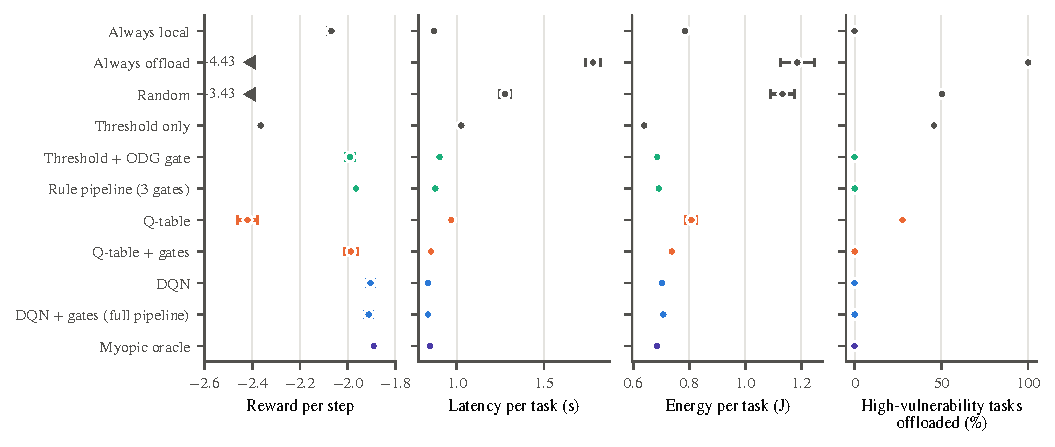
\includegraphics[width=\textwidth]{../results/figures/fig07_policies.pdf}
\caption{The policies of Table~\ref{tab:policies} on four metrics (dots: mean over \NSeeds{} seeds; bars: 95\% confidence interval, mostly smaller than the dots). Grey: simple baselines; green: rule-based gates; orange: Q-table; blue: DQN; violet: myopic oracle. Higher reward is better; lower latency, energy and high-vulnerability offloading are better. The two weakest policies in the reward panel lie outside the plotted range and are labelled with their values.}
\label{fig:policies}
\end{figure*}

\subsection{Learning Behaviour}
Fig.~\ref{fig:learning}a shows the reward of the greedy policy on fresh episodes during training. The DQN passes the rule pipeline after about four thousand steps and then stays within the band between the rule pipeline and the oracle. The Q-table starts at the level of always-local (its table is initially zero), drops, recovers briefly and then deteriorates as training continues, ending below always-local. So the Q-table has not converged to a good policy at the discount factor of 0.95, and the sum of its Q-values would have been a misleading indicator of progress. Fig.~\ref{fig:learning}b shows that the discount factor explains most of the difference: with $\gamma=0$ the Q-table reaches $\GamZeroQ$ and is close to the DQN ($\GamZeroDqn$), with $\gamma=0.5$ it reaches $\GamHalfQ$, and with $\gamma=0.95$ only $\GamNinetyQ$, while the DQN stays at about $\GamNinetyDqn$ for all three values (five seeds each). In this environment nearly all of the reward of a decision is immediate; the only delayed effect is the edge load. Bootstrapping on a coarse, aliased discretisation of the state is a likely reason why a long horizon hurts the table, but we did not test this explanation. The practical conclusion is that the DQN is far less sensitive to this hyperparameter, and that the comparison with the Q-table is only fair if $\gamma$ is tuned for it.

\begin{figure*}[t]
\centering
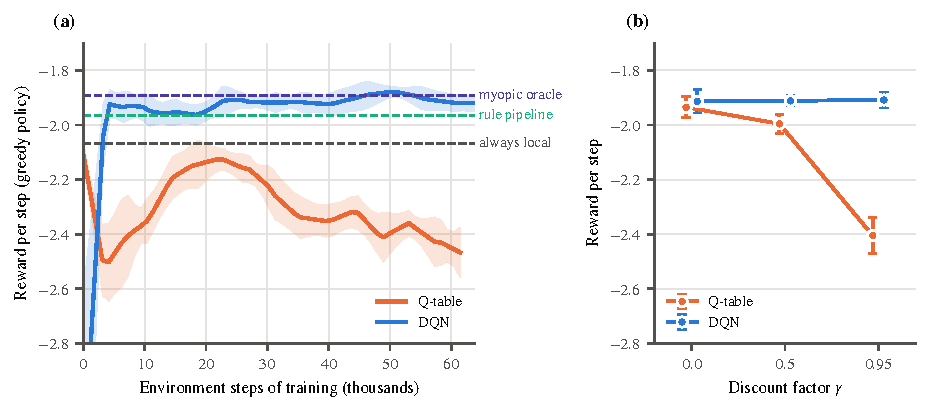
\includegraphics[width=\textwidth]{../results/figures/fig06_learning.pdf}
\caption{Learning behaviour. (a)~Reward per step of the greedy policy on fresh episodes versus the number of training steps, for the Q-table (orange) and the DQN (blue); lines are means over \NSeeds{} seeds and shaded bands the 95\% confidence interval. Dashed lines are the always-local policy, the rule pipeline and the myopic oracle (evaluation episodes of Table~\ref{tab:policies}). (b)~Final reward per step of the two agents for three discount factors (five seeds; bars: 95\% confidence interval).}
\label{fig:learning}
\end{figure*}

\subsection{Security of the Learned Policies}
The learned agents receive the vulnerability score as an input and a penalty for offloading, but nothing forces them to respect it. We therefore probed the trained agents, without any gate, on 20{,}000 states visited by a random policy and report the share of high-vulnerability states ($V\ge0.66$) in which they choose to offload (Table~\ref{tab:probe}). The Q-table offloads \ProbeQHigh\% of them on average (up to \ProbeQHighMax\% for some seed), whereas the DQN offloads none in any of the \NSeeds{} seeds, including in the subset of high-vulnerability states in which the bandwidth, complexity, battery and load otherwise favour offloading. This is a property of the particular environment: the security penalty ($3.0$) exceeds the largest possible latency benefit, so a well-trained agent has no incentive to offload such tasks. It is an empirical result for these agents rather than a guarantee, since the penalty is a soft constraint, and a different penalty weight or training run could behave differently. The hard ODG gate in front of the learned policy is therefore kept: it enforces the property by construction.

\begin{table}[t]
\caption{Share of states in which the trained agents choose to offload without any gate, on 20{,}000 states visited by a random policy (mean over \NSeeds{} seeds; range over seeds in parentheses). High vulnerability means $V\ge0.66$; ``fav.'' (favourable) additionally requires bandwidth above about 16~Mbps, complexity above 0.5, battery above 0.2 and edge load below 0.5.}
\label{tab:probe}
\centering
\footnotesize
\begin{tabular}{@{}lccc@{}}
\toprule
Agent & All states (\%) & High vuln.\ (\%) & High vuln., fav.\ (\%) \\
\midrule
Q-table & 40.1 & 33.4 (29.8--37.2) & 34.4 (9.8--52.7) \\
DQN & 16.4 & 0.0 (0.0--0.0) & 0.0 (0.0--0.0) \\
\bottomrule
\end{tabular}

\end{table}

\subsection{What the DQN Learned}
Fig.~\ref{fig:surfaces} shows the difference between the learned values of offloading and of local execution on three slices through the state space. In the first slice, the preference for offloading appears only at vulnerability below roughly 0.4 and at bandwidths above about 15--20~Mbps, close to the analytical thresholds of Eq.~\eqref{eq:threshold}; at higher vulnerability, local execution is preferred even at 100~Mbps. The third slice shows that the bandwidth at which offloading becomes preferable rises as the edge load increases, which is the effect of the queueing delay in the reward. In the second slice, offloading is preferred for complex tasks at high battery levels, and the preference weakens at very low battery levels and for light tasks. The weaker preference at very low battery was not designed into the reward and we did not investigate its cause. These surfaces show that the network reproduces the structure that the model implies; since the reward is derived from our own cost model, they do not show that this structure is the right one for a real system.

\begin{figure*}[t]
\centering
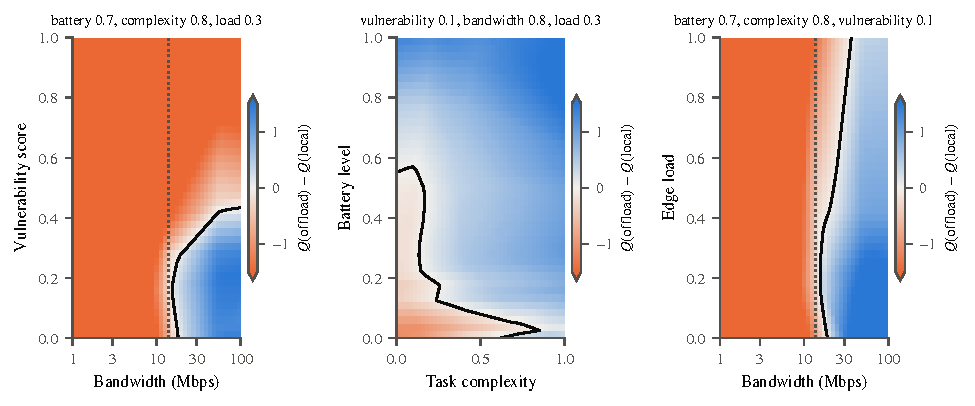
\includegraphics[width=\textwidth]{../results/figures/fig08_dqn_surfaces.pdf}
\caption{Learned DQN preference for offloading (seed 0) on three slices of the state space; colour shows $Q$(offload)$-Q$(local), clipped to $\pm1.5$ (blue: offloading preferred, orange: local execution preferred), and the black line is the decision boundary. (a)~Bandwidth versus vulnerability score at battery 0.7, complexity 0.8, load 0.3. (b)~Task complexity versus battery level at vulnerability 0.1, bandwidth 0.8 (normalised), load 0.3. (c)~Bandwidth versus edge load at battery 0.7, complexity 0.8, vulnerability 0.1. The dotted vertical line marks the analytical threshold $R^{*}=\RstarNoSetup$~Mbps.}
\label{fig:surfaces}
\end{figure*}

\subsection{Summary}
In the simulator, (i) the analytical threshold gives a clear first decision gate, (ii) a drift-plus-penalty admission controller bounds the edge queue and, at equal admission, collects more benefit than a fixed threshold, (iii) ODG gating keeps labelled sensitive objects on the device by construction, although the ratio score leaks transitively dependent objects, (iv) a DQN over the continuous state matches the myopic oracle and beats the rule pipeline by a small margin, and is more robust than a Q-table to the choice of discount factor, and (v) a hard gate in front of the learned policy is still advisable.

\section{Computational Complexity}
The analytical bandwidth threshold requires constant-time computation and therefore has complexity $O(1)$. The Q-Learning agent updates a single state-action pair at each interaction and its storage grows as $O(|S||A|)$ for $|S|$ states and $|A|$ actions; with the discretisation used here, $|S|=1{,}440$, but $|S|$ grows multiplicatively with every additional variable or bin. The ODG vulnerability analysis requires traversal of object relationships; for a graph with $V$ vertices and $E$ edges, scoring one object costs $O(V+E)$. The admission controller evaluates one comparison per arriving task, which is $O(1)$ per task. For the DQN, forward inference is proportional to the number of weights, $O(W)$ with $W=\DqnParams$ here. Although DQN training adds computational overhead compared with tabular Q-Learning (in our runs about 45 seconds per seed against a few seconds for the table), it removes the discretisation and was less sensitive to the discount factor.

\section{Limitations}
\label{sec:limitations}
\begin{itemize}
\item \textbf{Simulation only.} There is no real-device or real-network evaluation. Latency, energy and security trade-offs come from our own cost model, with assumed power and battery values; the reward the agents optimise is defined by that model.
\item \textbf{Workload proxy.} N-Queens stands in for CPU-bound tasks. Local times are measured on a desktop CPU and the edge time is modelled, not measured on a remote machine. In the policy experiments, tasks are abstract (complexity, data size) and do not run N-Queens.
\item \textbf{Single edge server.} Multi-server orchestration and load balancing are not considered, and the edge load is a scalar state.
\item \textbf{Learning problem.} Because the reward is derived from a known model and a decision affects later tasks mainly through the edge load, the learned policy largely matches a myopic optimum; the environment is only weakly sequential.
\item \textbf{Modest margins.} The learned policy beats the rule pipeline by about 3\% in reward; there is no comparison with algorithms from the literature or with real traces.
\item \textbf{Queue controller.} The drift-plus-penalty rule and its simple bound are evaluated on Poisson arrivals with bounded benefits; per-user fairness and heterogeneous service times are not modelled.
\item \textbf{ODG.} The example graph is hand-built, scores depend on how objects are labelled, and the ratio score can let objects with sensitive upstream dependencies offload. Random-graph results depend on the generator.
\item \textbf{Soft security constraint.} The security behaviour of the learned agents is empirical; only the hard gate gives a guarantee.
\item \textbf{Statistics.} \NSeeds{} seeds for the main comparison and five for the discount-factor study; confidence intervals use a $t$ distribution and assume approximate normality.
\end{itemize}

\section{Conclusion}
This paper studied a security-aware adaptive computation offloading framework for Mobile Edge Computing in simulation. The framework integrates an analytical bandwidth threshold, workload characterisation, reinforcement learning, Lyapunov drift-plus-penalty queue control, Object Dependency Graph vulnerability analysis, and Deep Q-Network-based continuous-state learning. The analytical model identified a break-even bandwidth of $\RstarNoSetup$~Mbps ($\RstarSetup$~Mbps with the connection setup delay). The drift-plus-penalty controller bounded the simulated edge queue by $Vb_\text{max}+A_\text{max}$, and in the deterministic illustration the throttled queue stayed at $\QCtrlDet$ tasks against $\QGreedyDet$ for greedy admission. ODG gating kept labelled sensitive objects on the device, and a comparison with a stricter taint rule quantified how much the ratio score leaks. The DQN matched a myopic oracle and improved on the rule pipeline by a small margin; the Q-table was much more sensitive to the discount factor, and the learned agents respected the security penalty in our experiments but without a guarantee. The results illustrate the design under simplified assumptions and are not evidence of performance on real systems.

\section{Future Scope}
Several extensions can further improve the work: evaluation on real Android and iOS devices and edge hardware, with measured latency and energy; comparison against offloading algorithms from the literature and real workload and bandwidth traces; multi-server edge orchestration and load balancing; per-user admission control with fairness; runtime Object Dependency Graph generation from real applications; federated reinforcement learning for collaborative policy learning; energy-harvesting-aware offloading; and explainable reinforcement learning for security-critical applications. Settings such as healthcare monitoring, industrial IoT and smart-city analytics are natural candidates for such studies, but they were not evaluated here.

\bibliographystyle{IEEEtran}
\bibliography{refs}

\EOD

\end{document}
